\documentclass[12pt]{article}

\usepackage[a4paper,margin=0.5in]{geometry}

\usepackage[square,numbers,sort&compress]{natbib}
%\usepackage[sort&compress]{natbib}

\usepackage[utf8]{inputenc} % allow utf-8 input
\usepackage[T1]{fontenc}    % use 8-bit T1 fonts
\usepackage{hyperref}       % hyperlinks
\usepackage{url}            % simple URL typesetting
\usepackage{booktabs}       % professional-quality tables
\usepackage{amsfonts}       % blackboard math symbols
\usepackage{nicefrac}       % compact symbols for 1/2, etc.
\usepackage{microtype}      % microtypography
\usepackage{amsmath}
\usepackage{algorithm}
\usepackage[noend]{algpseudocode}

\usepackage{times}
\usepackage{amsfonts}
\usepackage[psamsfonts]{amssymb}
\usepackage{latexsym}
\usepackage{color}
\usepackage{graphics}
\usepackage{enumerate}
\usepackage{amstext}
\usepackage{blkarray}
\usepackage{url}
\usepackage{epsfig}
\usepackage{bm}
\usepackage{hyperref}
\hypersetup{
    colorlinks=true,
    linkcolor=blue,
    filecolor=magenta,      
    urlcolor=blue,
}
\usepackage{mathtools}


\usepackage{graphicx}
\newcommand{\bigo}[1]{{\cal O}\left(#1 \right)}
\newcommand{\p}[1]{\mathrm{P}\left(#1 \right)}
\newcommand{\vect}[1]{\mathbf{#1}}
\newcommand{\tr}{^\mathrm{t}}
\newcommand{\matr}[1]{\bm{#1}}    

\begin{document}
\thispagestyle{empty}
\begin{center}

\textbf{DS-GA 3001.001 Special Topics in Data Science: Probabilistic Time Series Analysis\\
Homework 3}
\end{center}


\noindent \textbf{Due date: Oct 25, by 6pm}\\
\noindent YG390\\

\noindent \textbf{Problem 1.} (15p)\\
Consider the HMM with K=3 latent states and discrete observations $\{1,2,3\}$, with parameters specified by:
initial distribution $\pi = [1, \, 0,\, 0]$, 
transition matrix 
$ \mathbf{A} = \begin{bmatrix}
    0 & 0.5 & 0.5\\
    1 & 0 & 0 \\
    0 & 1 & 0
    \end{bmatrix}
$, where $A_{ij} = \mathrm{P}(z_{t+1}= j | z_t= i)$ 
and likelihood $\mathrm{P}(x_t|z_t)$ described by matrix entries $B_{xz}$:
$ \mathbf{B} =  \begin{bmatrix}
    0.5 & 0.5 & 0 \\
    0.5 & 0 & 0.5 \\
    0 & 0.5 & 0.5
    \end{bmatrix}.
    $\\
 Write down all possible state sequences consistent with observations a) 1, 2, 3 and b) 1, 3, 1.\\
Let the three latent states be $\{ S_1, S_2, S_3 \}$. Given the HMM with parameters $\{A,B,\pi\}$, the model can be described as:

\begin{center}
	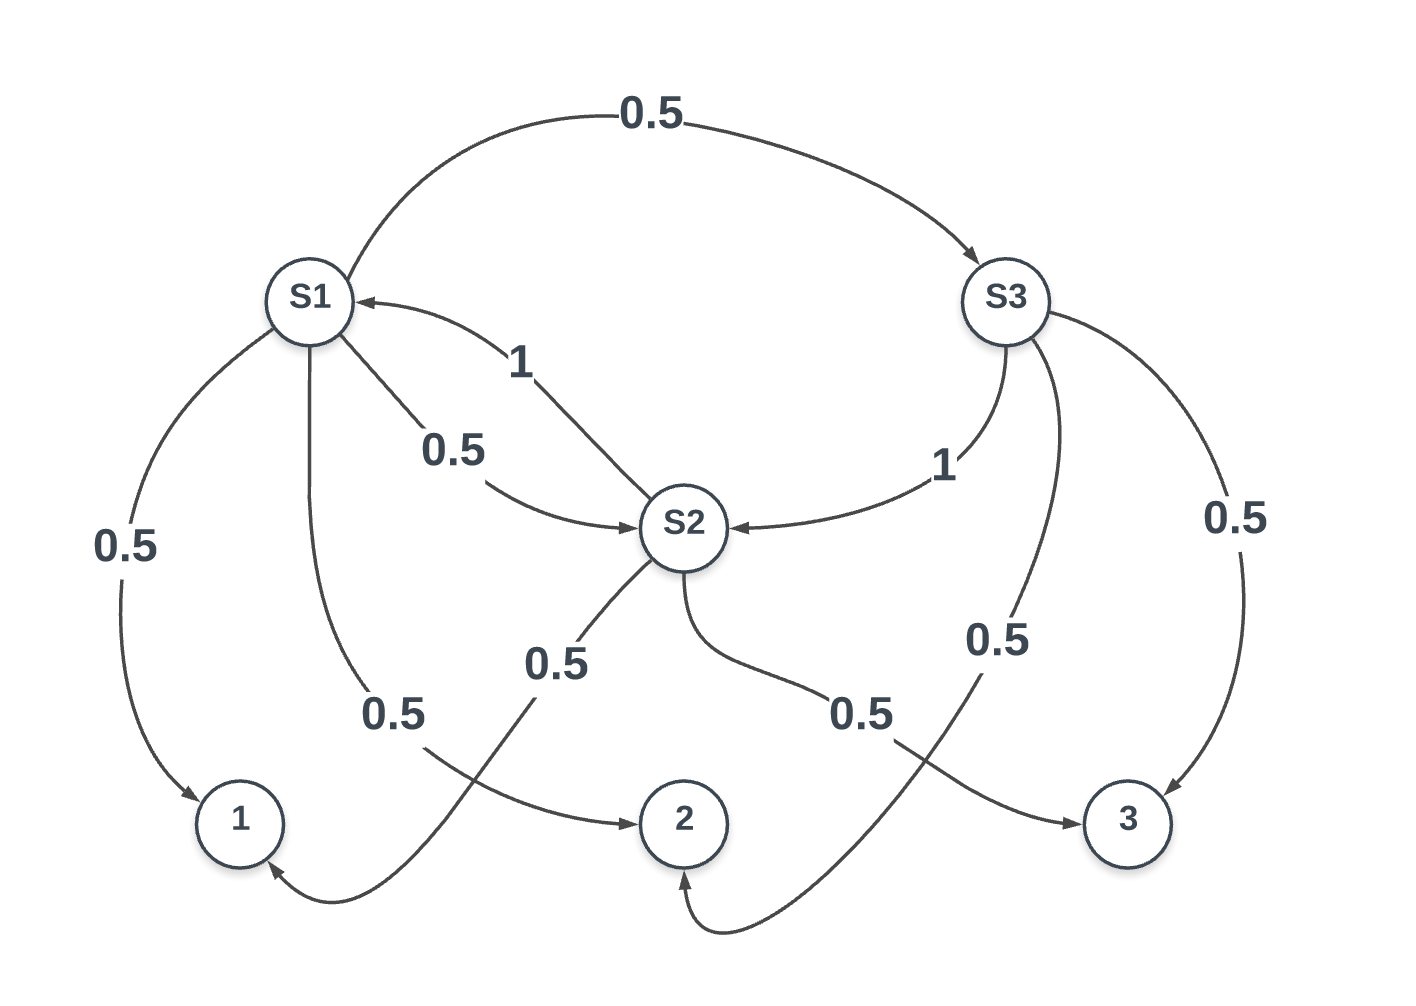
\includegraphics[width=1\linewidth]{figures/problem-1-1.png} 
\end{center}

When observing the observations 1,2, and 3 with initial distribution $\pi$ which implies we start in state $S_1$ then observing 2 means we have 0.5 probability of being in state $S_1$ or $S_3$.
However staying in state $S_1$ is not possible so the only state after seeing the sequence 1,2 is state $S_3$. Then the last observation 3 means we are in state $S_2$ or $S_3$. but from state $S_3$, 
the only existing transition is from $S_3$ to $S_2$. So the sequence of observations 1,2,3 corresponds to the state sequence $\{S_1, S_3, S_2 \}$.

When observing 1,2,1 with initial distribution $\pi$, seeing 2 after 1 implies we can be in state $S_2$ 50\% of the time or $S_3$ the rest of the time. The last observation 1 implies that the latent space is either $S_1$ or $S_2$.
Based on the transition matrix $\matr{A}$ then the only possible state sequences for the sequence of observations $\{1,2,1\}$ are $\{S_1, S_2, S_1\}$ or  $\{S_1, S_3, S_2\}$.

\noindent \textbf{Problem 2.} (15p)\\
Construct an HMM that generates the observation sequence $A^{k_1}C^{k_2}A^{k_3}C^{k_4}$ where $A^{k_1}$ denotes $k_1$ repeats of symbol $A$ and the number of repeats $k_i$ are drawn from the set $\{1,2,3\}$ with equal probability.\\

The HMM model is defined by three class of parameters $\{\matr{A}, \matr{B}, \pi \}$, and is described in the graph below. Note that there is a direct connection between the states STOP\_k2 and S\_7 which I broke down into two for convenience of
representation.
The latent states are $\{S_1, S_2, S_3, S_4, S_5, S_6, S_7, S_8, S_9, S_{10}, S_{11}, S_{12}\}$. Sequences based on $k_i$ have equal probability $\frac{1}{3}$, meaning, that for example for $k_1$: A, AA, AAA have the same probability $\frac{1}{3}$.
The transition matrix has for elements the probabilities indicated on the graph and $\sum_{j} A_{ij}=1$.

$$B_{ih}=\frac{num\ of\ times\ state\ i\ emits\ h}{num\ state\ i}$$
The emission probabilities $\matr{B}$, is the identity matrix since there are as many observations repeated for A,
then the number of state $S_i$, and the same for C and $S_j$.
$$\pi_{i}=\frac{num\ of\ chains\ start\ with\ i}{total\ num\ of\ chains}$$
All the chains start with a sequence of A in $S_1$, the initial distribution is $\pi = [1 0 0 0 0 0 0 0 0 0 0 0]^T$.

\begin{center}
	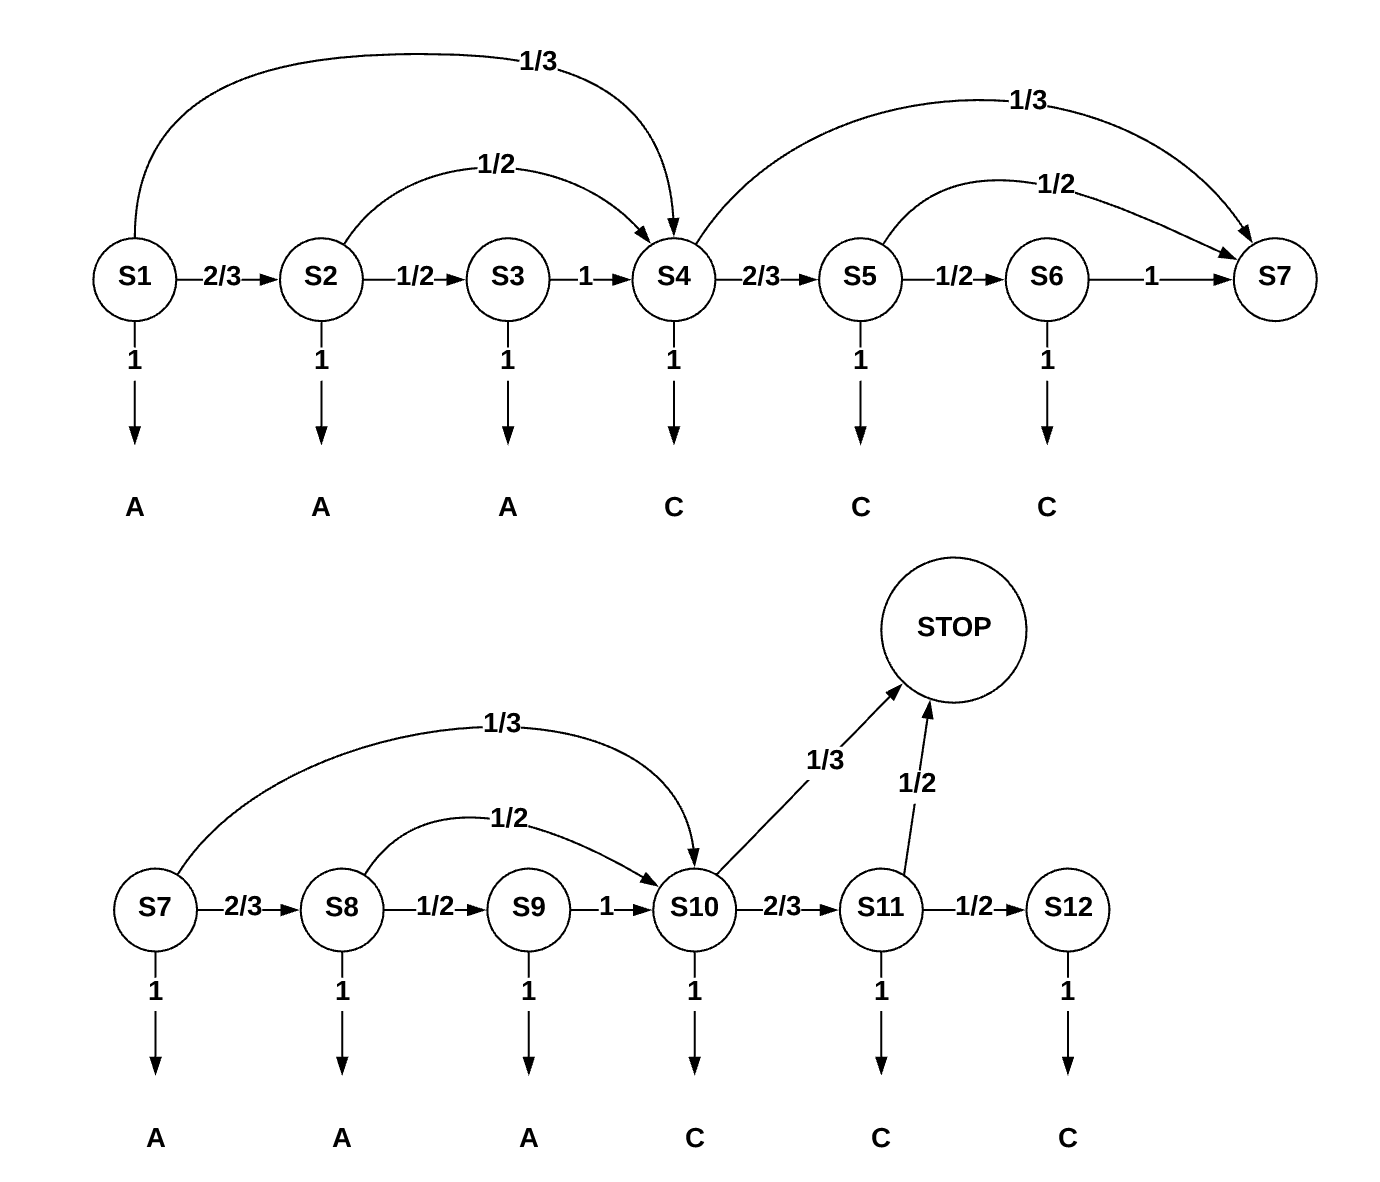
\includegraphics[width=1\linewidth]{figures/problem-2-2.png} 
\end{center}


\noindent \textbf{Problem 3.}  (20p)\\ 
Implement EM for an HMM model with K states and gaussian observations (full derivations in handout). 
Use this code to fit the weekly S\&P 500 returns data (data/sp500w.csv) for K = 2 vs. K = 3 and compare the two results. \\
Hint: Use Example 6.17 from tsa4 textbook as guideline for plots and interpretation.


For the parameters initialization:
\begin{enumerate}
	\item We use a gaussian mixture which gives us estimates for the mean and the covariance of each components namely $\mu_k$ and $\Sigma_k$ from
the handout.
	\item  The initial distribution of the initial state $\vect{z}_1$, $\vect{\pi}$ is estimated by implementing an expectation step on the data itself and computing $\pi=\p{\vect{z}_1|\vect{x}_1}$. 
	\item Based on the KMeans algorithm that we implemented, we obtain a label for every point of the dataset. We then use this labeling to approximate the initial transition matrix, by counting the number of transition among labels 
and normalizing the frequencies.
\end{enumerate}

This is the plot of the S\&P 500 returns over many years with estimated labels:
\begin{center}
	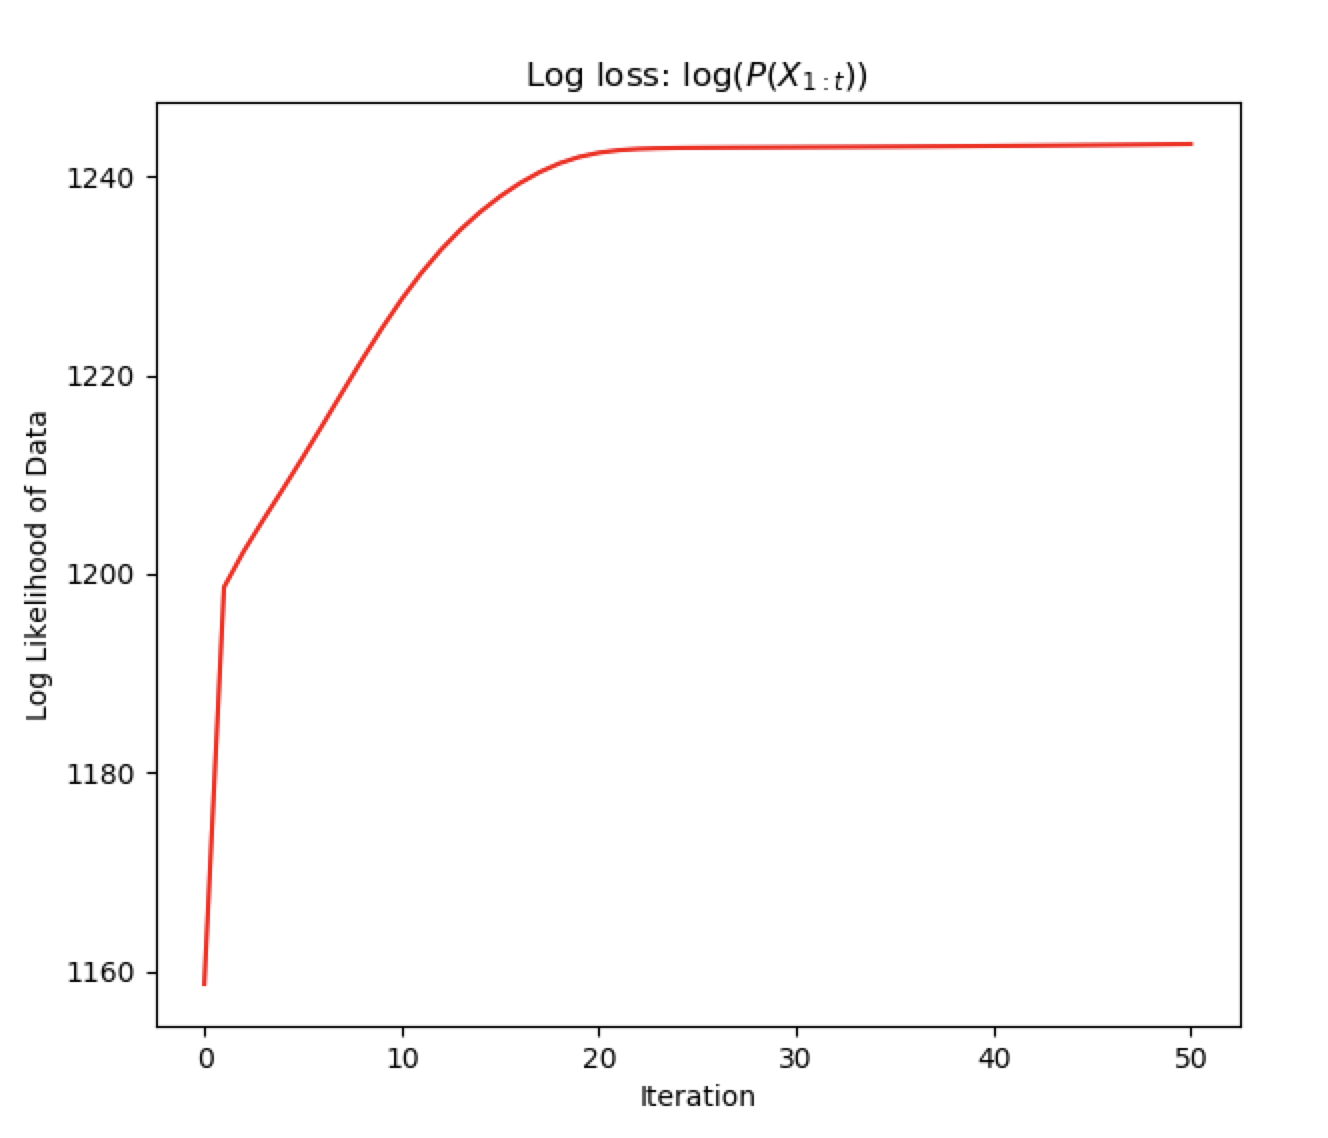
\includegraphics[width=1\linewidth]{figures/problem-3-1.png} 
\end{center}

Once the initialization is completed, we alternate between the E steps, for which we run the alpha-beta algorithm with the current estimates, determining:
\begin{align*}
	\hat{\alpha}(\vect{z}_i)			&=	\p{\vect{z}_i | \vect{x}_{1:i}} 	=	\frac{\alpha(\vect{z}_i)} {\p{ \vect{x}_{1:i} }}	\\
	\hat{\beta}(\vect{z}_i)				&=	\frac{ \p{ \vect{x}_{i+1:t} | \vect{z}_i } }  {\p{ \vect{x}_{i+1:t} |  \vect{x}_{1:i}}}	= \frac{ \beta(\vect{z}_i) } {\Pi _{j=i+1:t} c_j} \\
	\gamma(\vect{z}_i)				&= 	\hat{\alpha}(\vect{z}_i) \hat{\beta}(\vect{z}_i)	\\
	\xi(\vect{z}_{i,j}, \vect{z}_{i+1,k})	&= 	c_{i+1}^{-1} \hat{\alpha}(\vect{z}_i) \p{\vect{z}_{i+1} | \vect{z}_i} \p{\vect{x}_{i+1} | \vect{z}_{i+1}} \hat{\beta}(\vect{z}_{i+1})	
\end{align*}

And the M step, which updates the parameters:
\begin{align*}
	\pi_k			&=	\frac{ \gamma(\vect{z}_{1,k}) } {\sum_j \gamma(\vect{z}_{1,j}) } \\
	\matr{A}_{jk}	&=	\frac{ \sum_i \xi(\vect{z}_{i,j} , \vect{z}_{i+1,k})}	{ \sum_{i,l} \xi(\vect{z}_{i,j} , \vect{z}_{i+1,l}) } \\
	\mu_k		&=	\frac{1} {\sum_i \gamma(\vect{z}_{i,k}) }  \sum_i \gamma(\vect{z}_{i,k}) \vect{x}_i \\
	\Sigma_k		&= 	\frac{1} {\sum_i \gamma(\vect{z}_{i,k}) }  \bigg(	\sum_i \gamma(\vect{z}_{i,k}) \vect{x}_i  \vect{x}_i^t	\bigg) - \mu_k \mu_k^t
\end{align*}

The result for $K=3$, are plotted below with the top plot showing the log loss of the data, the middle plot the inference obtained with our model and at the bottom, the plot using the means and covariances
indicated by ts4 textbook.  We can see that our model, to some extent, captures better the distribution of the raw data.

\begin{center}
	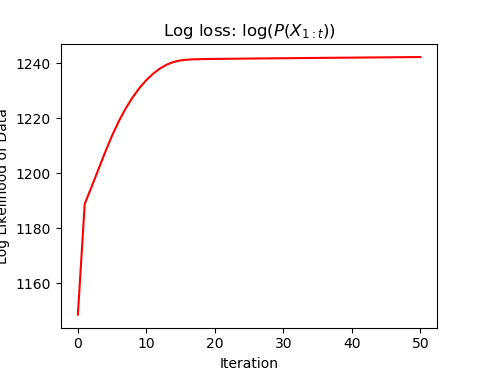
\includegraphics[width=1\linewidth]{figures/problem-3-2.png} 
\end{center}

\begin{center}
	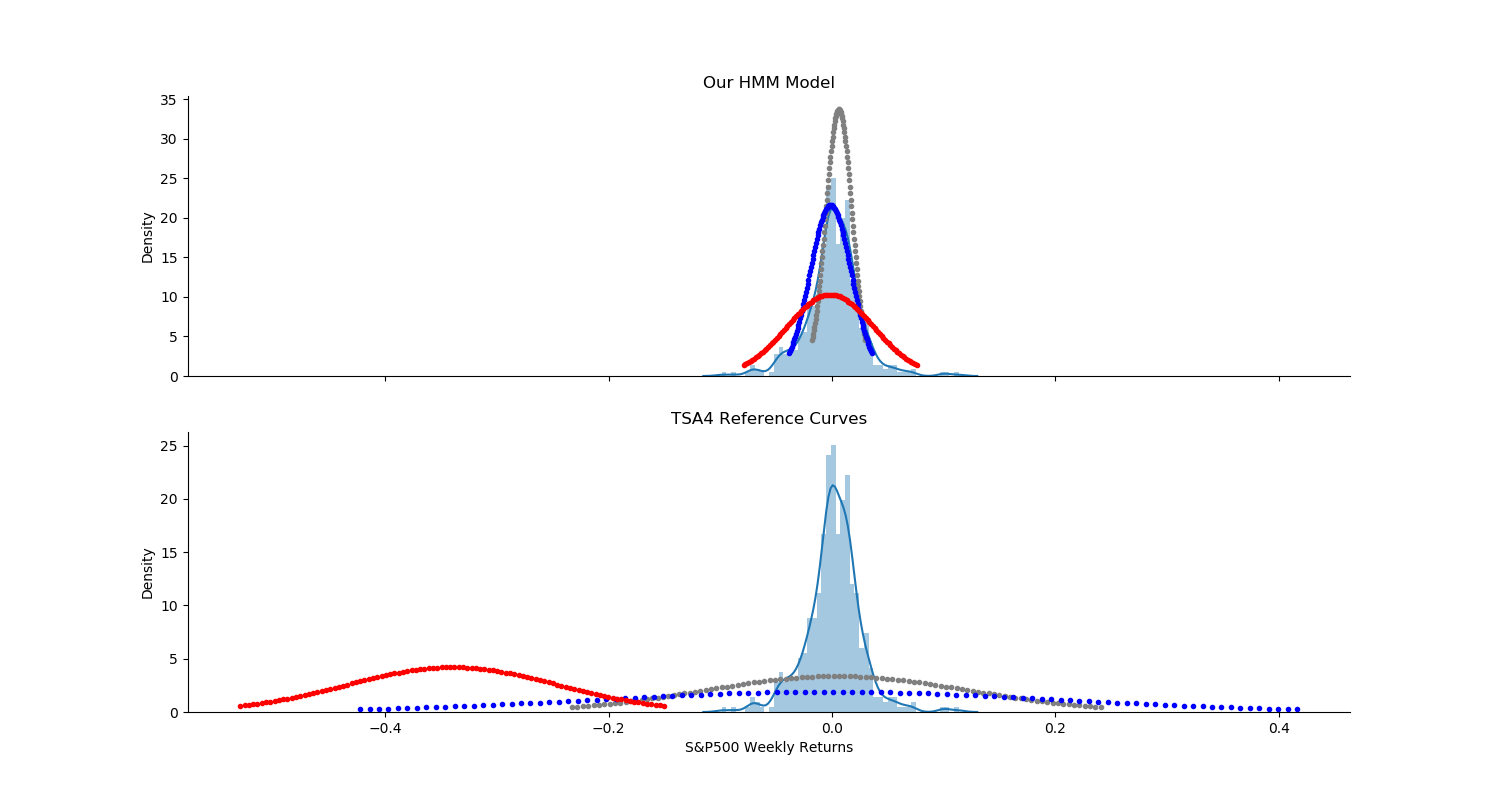
\includegraphics[width=1\linewidth]{figures/problem-3-3.png} 
\end{center}

The performance of our model compared to hmmlearn Gaussian smoother,  are similar, the GaussianHMM model covering more of the data along the x-axis whereas our model covers the
distribution better along the y-axis.
\begin{center}
	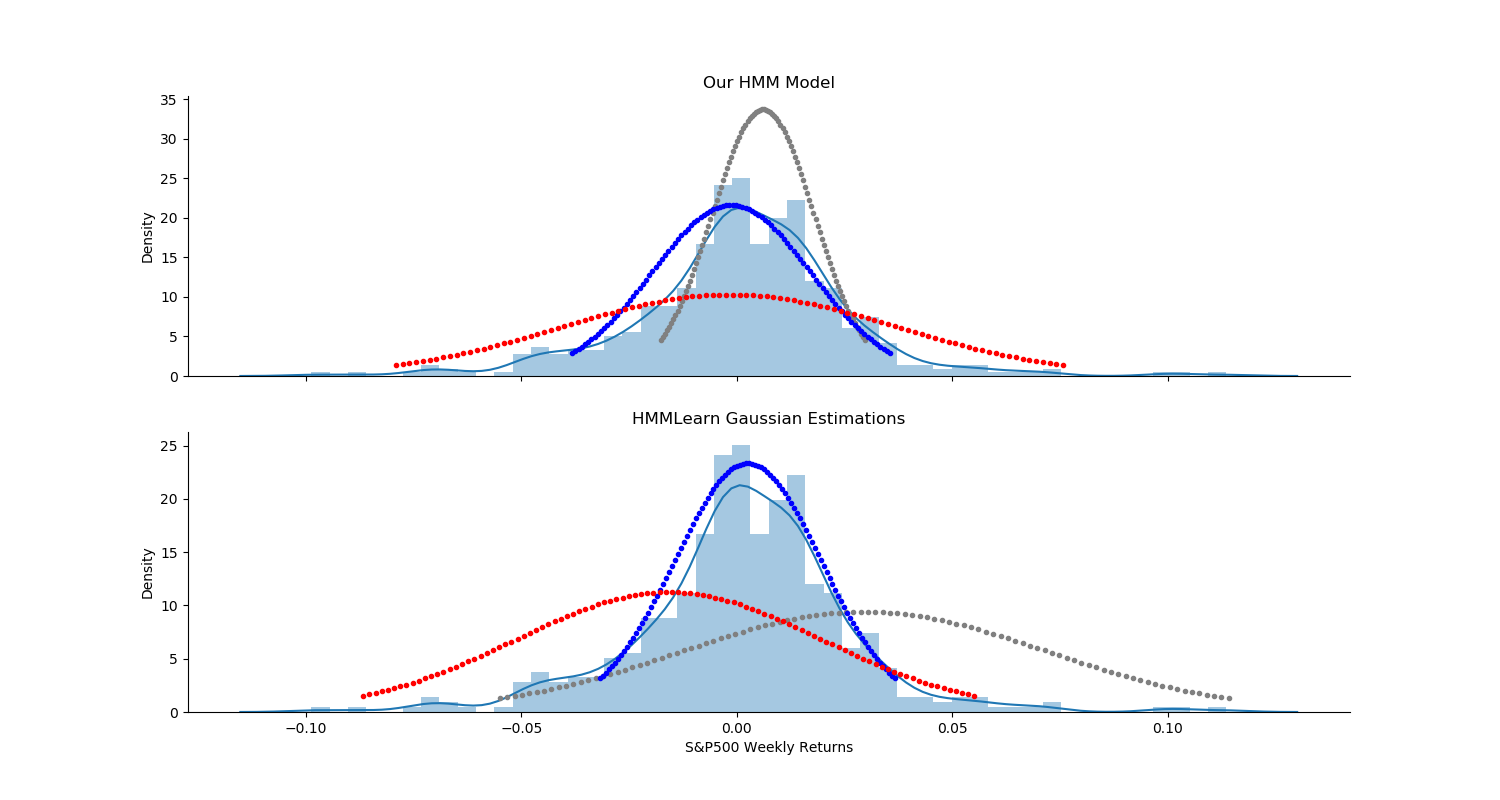
\includegraphics[width=1\linewidth]{figures/problem-3-4.png} 
\end{center}

For $K=2$, the fit is worst but we can see that tsa4 model does not cover the distribution along the y-axis. 
Compared to hmmlearn gaussian model, our model performance is very similar.

\begin{center}
	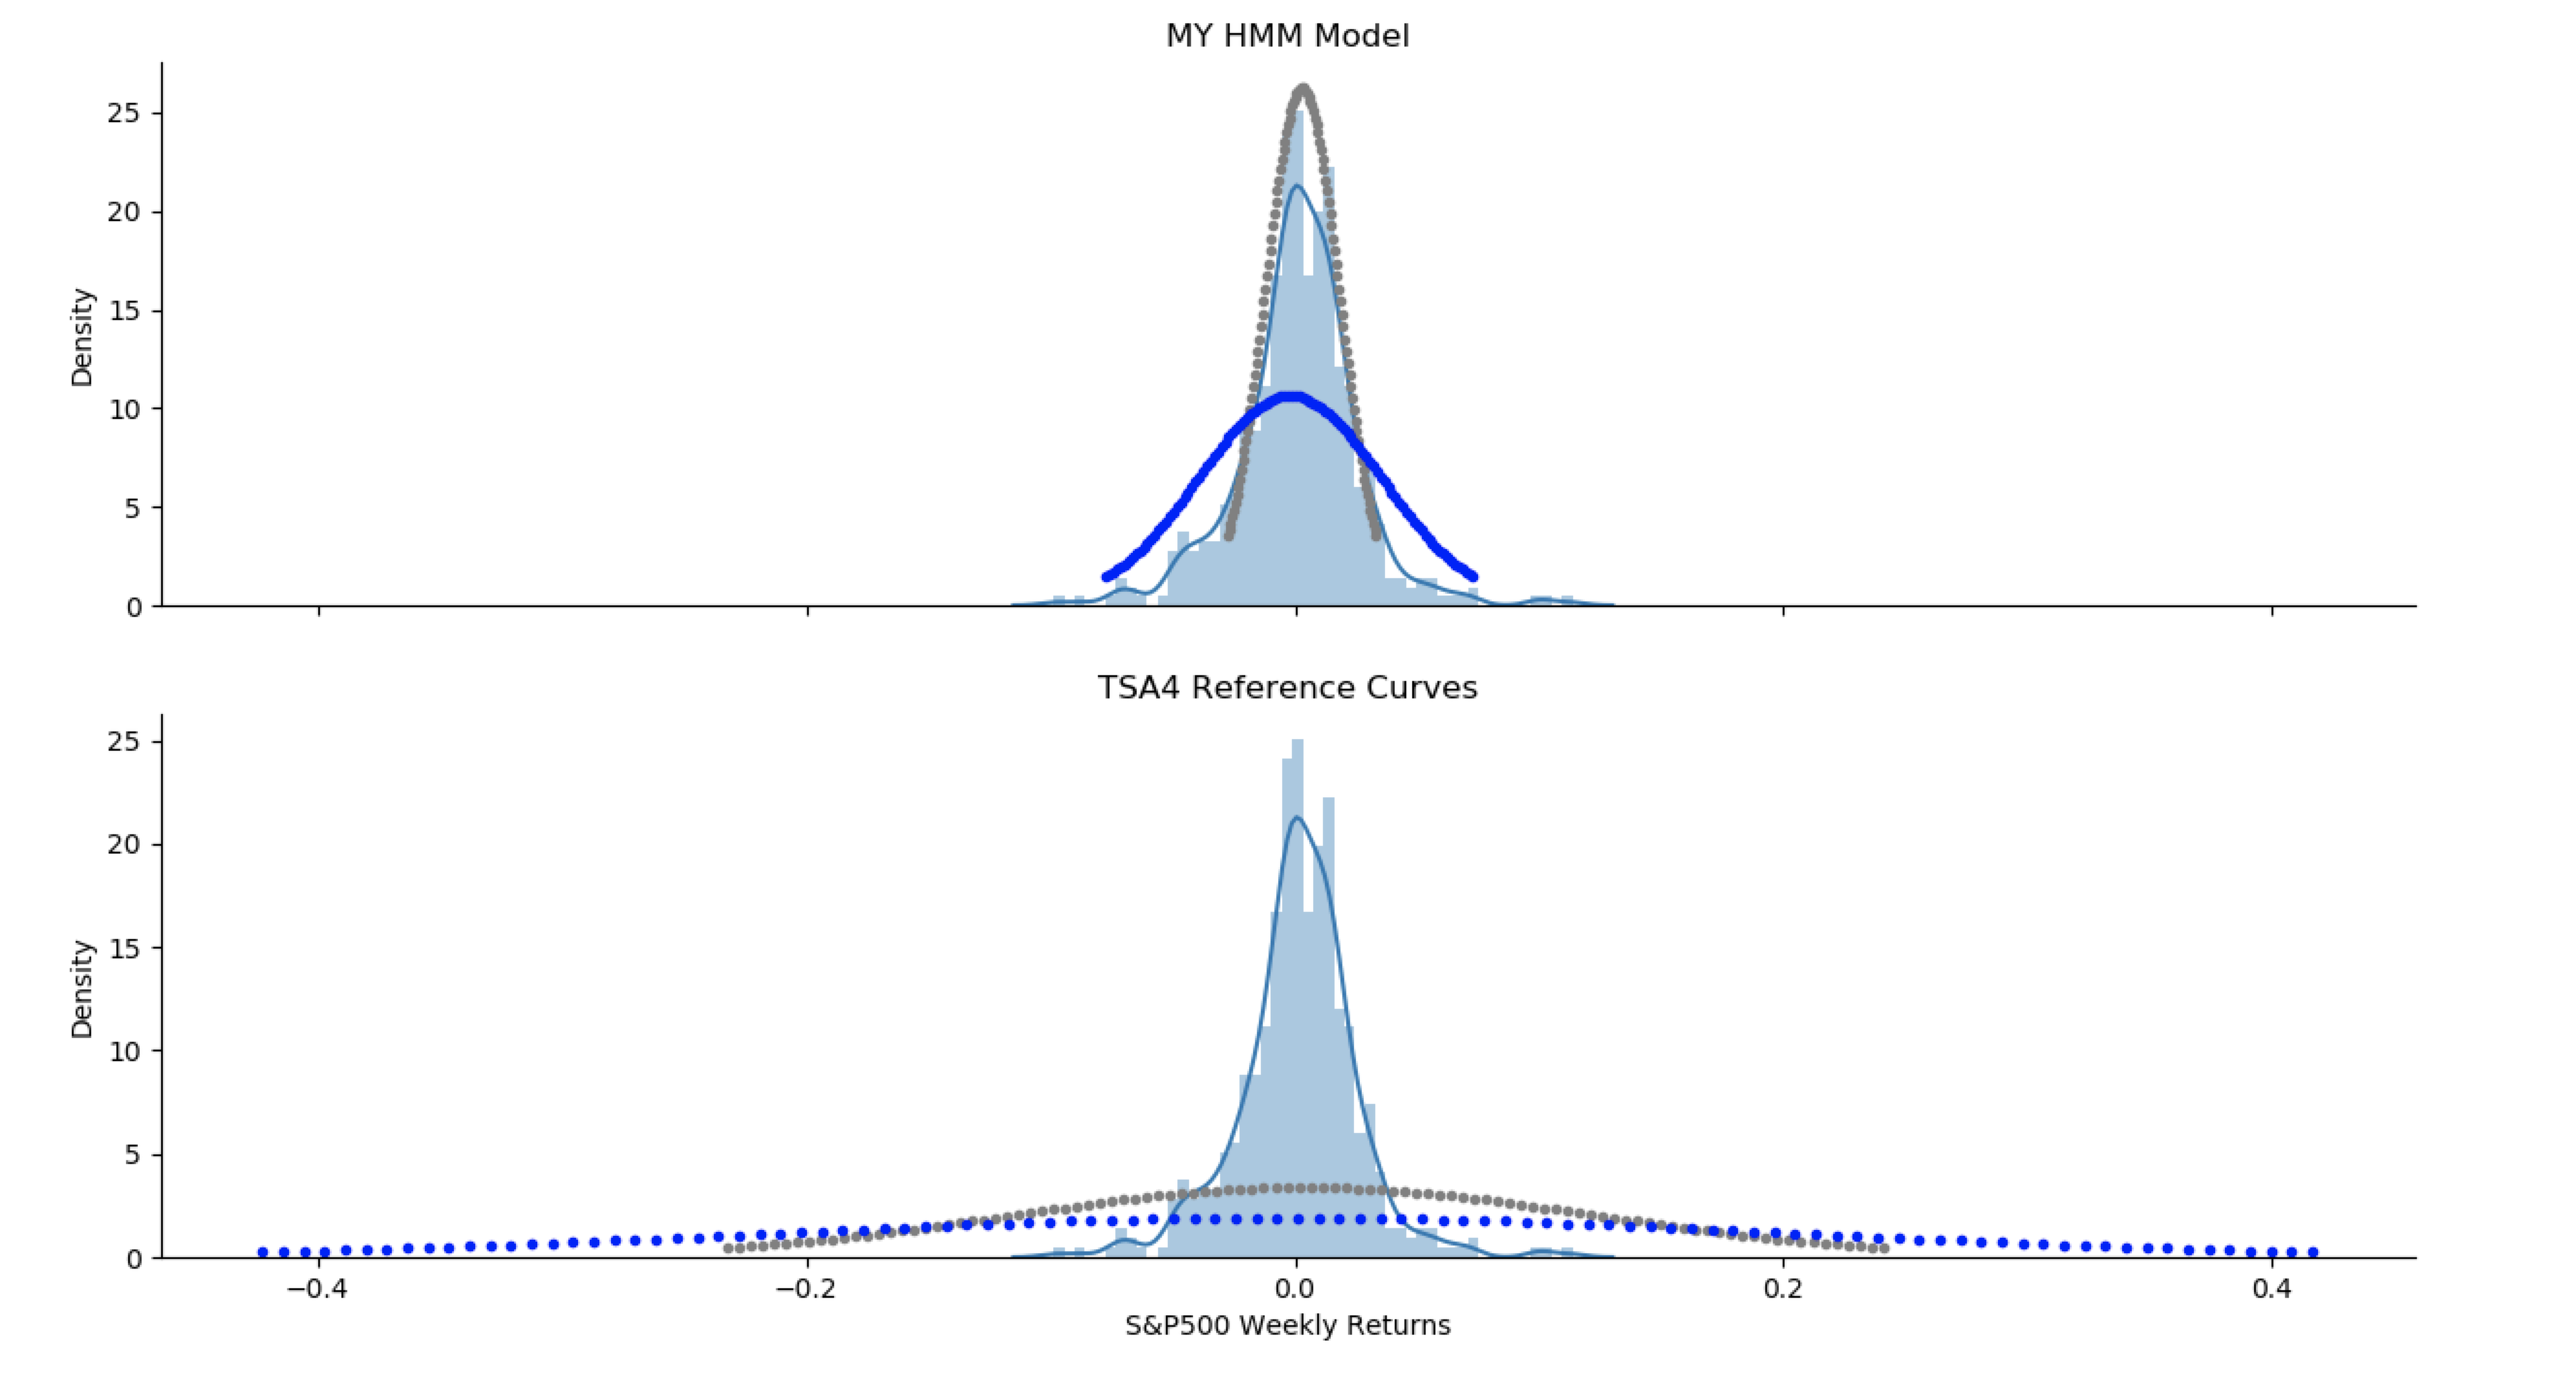
\includegraphics[width=1\linewidth]{figures/problem-3-5.png} 
\end{center}

\begin{center}
	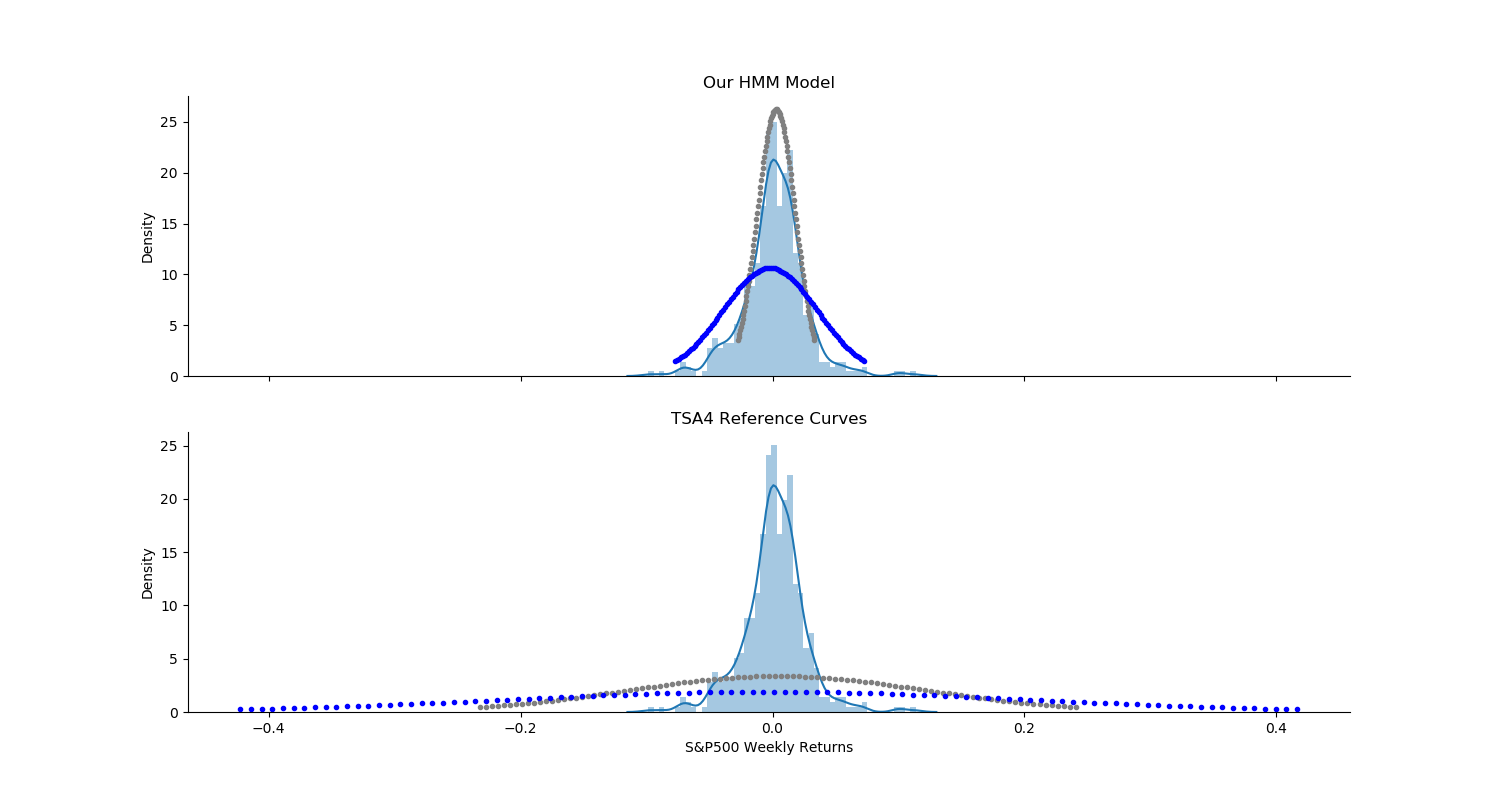
\includegraphics[width=1\linewidth]{figures/problem-3-6.png} 
\end{center}

\begin{center}
	\includegraphics[width=1\linewidth]{figures/problem-3-7.png} 
\end{center}

\end{document}